\documentclass{article}

\usepackage{graphicx}
\usepackage{tikz}
\usepackage{tikzsymbols}
\usetikzlibrary{calc,patterns,shapes.geometric}
\pagestyle{empty}
\usepackage[margin=0pt]{geometry}
\geometry{papersize={14in,12in}}

\def\centerarc[#1](#2)(#3:#4:#5){\draw[#1] ($(#2)+({#5*cos(#3)},{#5*sin(#3)})$) arc (#3:#4:#5);}

\begin{document}
	\begin{figure}
		\centering
		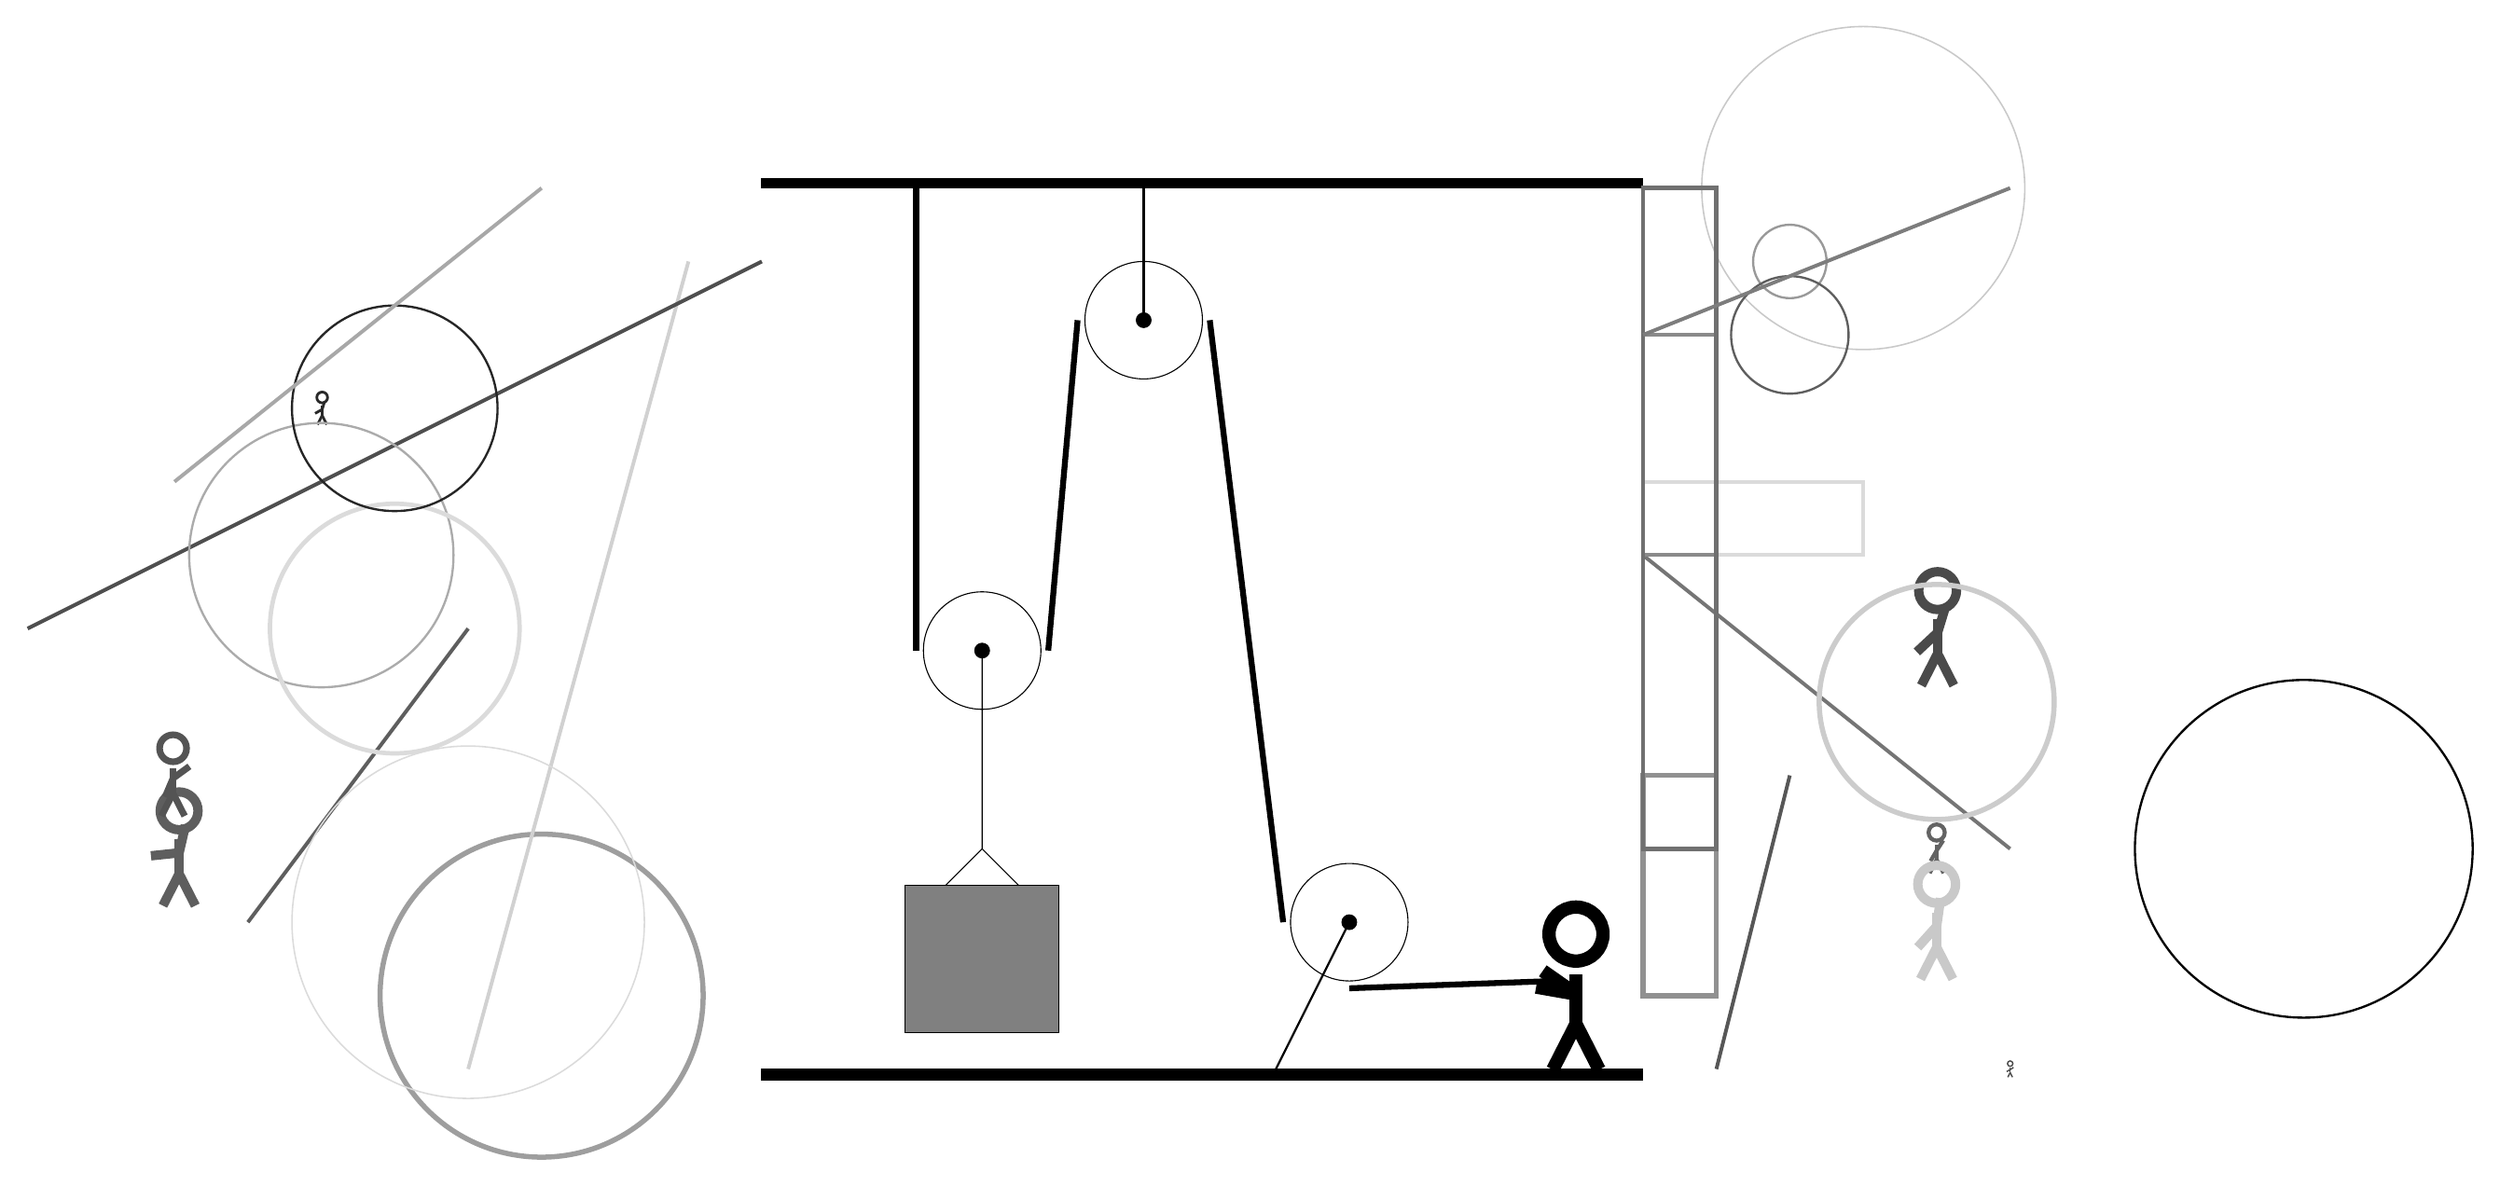
\begin{tikzpicture}
			%%%%% START %%%%%
			
			\draw[fill=black] (-2, 9) rectangle (10, 9.125);
			
			\draw (3.2, 7.2) circle (0.8);
			\draw[fill=black] (3.2, 7.2) circle (0.1);
			\draw[thick] (3.2, 7.2) -- (3.2, 9);
			
			\draw (6, -1) circle (0.8);
			\draw[fill=black] (6, -1) circle (0.1);
			\draw[thick] (6, -1) -- (5, -3);
			
			\draw (1, 2.7) circle (0.8);
			\draw[fill=black] (1, 2.7) circle (0.1);
			
			\draw (1, 2.7) -- (1, 0) -- (0.5, -0.5);
			\draw (1, 0) -- (1.5, -0.5);
			\draw[fill=black!50] (-0.05, -0.5) rectangle (2.05, -2.5);
			
			\draw[line width=0.8mm] (0.1, 9) -- (0.1, 2.7);
			\centerarc[line width=0.8mm](1, 2.7)(180:360:0.9);
			\draw[line width=0.8mm](1.9, 2.7) -- (2.3, 7.2);
			\centerarc[line width=0.8mm](3.2, 7.2)(0:180:0.9);
			\draw[line width=0.8mm](4.1, 7.2) -- (5.1, -1);
			\centerarc[line width=0.8mm](6, -1)(180:270:0.9);
			\draw[line width=0.8mm](6, -1.9) -- (8.8, -1.8);
			
			\node at (9, -1.9) {\Strichmaxerl[10][-35][170]};
			
			\node[line width=0.3mm, color=black!71] at (14, 3) {\Strichmaxerl[7][43][73]};
			
			\node[line width=0.4mm, color=black!84] at (-8, 6) {\Strichmaxerl[2][29][73]};
			\draw [line width=0.2mm, color=black!21](13, 9) circle (2.2);
			\draw [line width=0.3mm, color=black!99](19, 0) circle (2.3);
			\draw [line width=0.3mm, color=black!40](12, 8) circle (0.5);
			
			\draw [line width=0.7mm, color=black!38](-5, -2) circle (2.2);
			
			\node[line width=0.6mm, color=black!63] at (-10, 0) {\Strichmaxerl[7][6][77]};
			\draw[line width=0.7mm, color=black!43] (10, -2) rectangle (11, 1);
			\node[line width=0.3mm, color=black!67] at (-10, 1) {\Strichmaxerl[5][67][36]};
			\draw[line width=0.5mm, color=black!14] (10, 5) rectangle (13, 4);
			\draw[line width=0.5mm, color=black!54](10, 4) -- (15, 0);
			\draw [line width=0.3mm, color=black!63](12, 7) circle (0.8);
			\draw[line width=0.5mm, color=black!18](-6, -3) -- (-3, 8);
			
			\draw[line width=0.5mm, color=black!63](-6, 3) -- (-9, -1);
			\draw[line width=0.5mm, color=black!46] (10, 7) rectangle (11, 4);
			\draw[line width=0.6mm, color=black!56] (11, 0) rectangle (10, 9);
			
			\draw [line width=0.7mm, color=black!20](14, 2) circle (1.6);
			\node[line width=0.4mm, color=black!71] at (15, -3) {\Strichmaxerl[1][29][34]};
			\draw[line width=0.5mm, color=black!69](-2, 8) -- (-12, 3);
			\draw [line width=0.2mm, color=black!14](-6, -1) circle (2.4);
			\draw [line width=0.3mm, color=black!33](-8, 4) circle (1.8);
			
			\draw [line width=0.6mm, color=black!14](-7, 3) circle (1.7);
			\draw[line width=0.5mm, color=black!51](15, 9) -- (10, 7);
			\draw [line width=0.3mm, color=black!85](-7, 6) circle (1.4);
			\node[line width=0.5mm, color=black!61] at (14, 0) {\Strichmaxerl[3][60][57]};
			\node[line width=0.5mm, color=black!21] at (14, -1) {\Strichmaxerl[7][48][82]};
			\draw[line width=0.5mm, color=black!66](11, -3) -- (12, 1);
			\draw[line width=0.5mm, color=black!34](-5, 9) -- (-10, 5);
			
			
			\draw[fill=black] (-2, -3) rectangle (10, -3.15);
			
			%%%%% END %%%%%
		\end{tikzpicture}
	\end{figure}	
\end{document}